
\documentclass[10pt, twocolumn, reqno, a4paper,oneside]{amsart}

\rmfamily{\fontsize{10pt}{\baselineskip}\selectfont}

% \usepackage[utf8]{inputenc}
\setlength{\columnsep}{4ex}
\usepackage{graphicx}
\usepackage{tikz}
\usepackage{color}
\usepackage[colorlinks=true, allcolors=blue]{hyperref}
\usepackage{xcolor}
\usepackage[top=2.3cm,bottom=1.8cm,left=1.4cm,right=1.4cm]{geometry}
\usepackage{amsfonts, amssymb, amsbsy}
\usepackage{environments}
\usepackage{amsthm,thmtools}
\usepackage{pgfplotstable}
\usepackage{booktabs}
\numberwithin{equation}{section}
\numberwithin{theorem}{section}
\numberwithin{figure}{section}
\numberwithin{table}{section}
\usepackage{mathrsfs}
\usepackage{subcaption}
\usepackage{bm}
\usepackage{physics}
\usepackage[normalem]{ulem}
\usepackage{listings}
\usepackage{algpseudocode}
\usepackage{algorithm, algorithmicx}
\numberwithin{theorem}{section}
\numberwithin{equation}{section}
% \numberwithin{remark}{section}
\lstset{basicstyle=\ttfamily}
\newenvironment{sketchoftheproof}{\paragraph{\textit{Sketch of the Proof}}}{\hfill$\square$}
\usepackage{caption}
\captionsetup{width=0.95\linewidth}

\newcommand\tbbint{{-\mkern -16mu\int}}
\newcommand\tbint{{\mathchar '26\mkern -14mu\int}}
\newcommand\dbbint{{-\mkern -19mu\int}}
\newcommand\dbint{{\mathchar '26\mkern -18mu\int}}
\newcommand\bint{
{\mathchoice{\dbint}{\tbint}{\tbint}{\tbint}}
}
\newcommand\bbint{
{\mathchoice{\dbbint}{\tbbint}{\tbbint}{\tbbint}}
}

\renewcommand{\algorithmicrequire}{\textbf{Input:}}
\renewcommand{\algorithmicensure}{\textbf{Output:}}
\newcommand{\cmrfont}[1]{{\fontfamily{cmr}\selectfont #1}}
\DeclareMathOperator*{\argmax}{arg\,max}
\DeclareMathOperator*{\argmin}{arg\,min}
\DeclareMathOperator*{\minimize}{minimize}
%\DeclareMathOperator*{\max}{max}

\makeatletter
\renewcommand\subsubsection{\@startsection{subsubsection}{3}{\z@}%
{-3.25ex\@plus -1ex \@minus -.2ex}%
{1.5ex \@plus .2ex}%
{\normalfont\normalsize\bfseries}}
\makeatother

\definecolor{darkgreen}{rgb}{0.0, 0.5, 0.0} % RGB for dark green

\hypersetup{
colorlinks,
linkcolor=green, % color of internal links (change box color with linkbordercolor)
citecolor=green, % color of links to bibliography
filecolor=magenta, % color of file links
urlcolor=cyan % color of external links
}


\title{A review of the Conditional Gradient method and a few applications}

\author{Tina Torabi}
\address{Tina Torabi\\
Department of Mathematics\\
University of British Columbia\\
1984 Mathematics Road\\
Vancouver, British Columbia\\
Canada
}
\email{torabit@math.ubc.ca}

\author{Alireza Yazdani}
\address{Alireza Yazdani\\
Department of Mathematics\\
University of British Columbia\\
1984 Mathematics Road\\
Vancouver, British Columbia\\
Canada
}
\email{ayazdani@math.ubc.ca}

\date{\today}

\begin{document}
\twocolumn[
\begin{@twocolumnfalse}
	\begin{abstract}
		This study explores the application of the conditional gradient method and its various adaptations as effective optimization strategies in the areas of Matrix Completion and feature selection, which are crucial in machine learning, statistics, and signal processing. The report not only highlights the effectiveness of the Conditional Gradient Method in addressing these vital challenges but also offers an in-depth comparative analysis of its different variants.
	\end{abstract}
	\maketitle
\end{@twocolumnfalse}
]


\section{Introduction}
\label{sec:intro}

The rapid growth of data-driven applications in various fields has given rise to a variety of optimization problems that demand efficient and scalable solutions. Among these, Matrix Completion and feature selection problems play a pivotal role in machine learning, statistics, and signal processing. This report presents an exploration of the conditional gradient method and its variants as a powerful optimization technique for tackling both of these problems.
First, consider a scenario where a matrix is given with only a subset of its entries known, and the task is to infer the missing entries. This problem, in its raw form, is ill-posed due to the absence of initial information about the matrix. However, matrices derived from real-world data frequently demonstrate inherent low-dimensional structures, offering a means to effectively constrain the solution space.
In recommender systems, when two users share a common interest in certain products, it is probable that they will exhibit a similar level of interest when encountering a new product, reflecting the existence of a low-rank structure in the user-item interaction matrix.
Low-rank matrix completion is a recurring problem in a variety of applications including recommendation systems \cite{6389682}, computer vision \cite{8265431}, and signal processing \cite{Li2019ASO}. The Netflix Prize Challenge \cite{Bennett2007TheNP} serves as an essential example and a motivating application for the study of low-rank matrix completion problems. Launched by Netflix, this competition aimed to improve the accuracy of predictions about how much a user would enjoy a film based on their previous ratings. The underlying challenge was to fill in a massive, sparsely populated matrix representing user ratings for various movies. Each entry in this matrix corresponded to a user's rating for a particular movie, but a vast majority of these entries were missing, as no user had rated all the movies in the database.  The question now arises: \textit {is it feasible to complete a matrix with partially observed entries given its rank is small?} In Section \ref{sec:MC}, we will rigorously formulate the low-rank matrix completion problem and discuss a well-established heuristic for solving it, as proposed by Fazel et al \cite{Fazel2002MatrixRank}. We will then compare two specific approaches in solving this problem using the conditional gradient method, by presenting and evaluating numerical results.

Now consider a complex machine learning project with a dataset that encompasses a wide array of features. In this high-dimensional data space, not all features contribute equally to the predictive accuracy of the model. Some may be crucial, while others could be redundant or even detrimental to the model's performance. This is where the concept of feature selection becomes indispensable. Among various feature selection techniques, Lasso (Least Absolute Shrinkage and Selection Operator), introduced by Tibshirani \cite{tibshirani1996regression}, excels in scenarios with high-dimensional datasets. In Section \ref{sec:lasso}, we will address this problem using the conditional gradient algorithm and provide numerical results to illustrate its practical applications.



\subsection*{Notation}

Let $\mathbb{R}^{m \times n}$ denote the space of all $m \times n$ real matrices. For a matrix $X \in \mathbb{R}^{m \times n}$, $X_{ij}$ represents the entry in the $i$-th row and $j$-th column.
Throughout this paper, $\langle X, Y \rangle$ denotes the inner product between two matrices $X$ and $Y$, defined as
$$\langle X, Y \rangle = \text{Tr}(X^\top Y)~=~ \sum_{i=1}^m\sum_{j=1}^n X_{ij}Y_{ij}$$, where $X^\top$ represents the transpose of $X$.
The Frobenius norm, denoted as $\| \cdot \|_F$, is the norm associated with this inner product,
$\|X\|_F~=~\text{Tr}(X^\top X)$.

The $i$-th largest singular value of $X$ is represented by $\sigma_i(X)$ which is equal to the square root of the $i$-th largest eigenvalue of $XX^\top$. The largest singular value of a matrix, denoted as $\|X\|$, is its operator norm or induced $2$-norm, which can be represented as
$\|X\| := \sigma_1(X).$
The rank of $X$, denoted as $r$, corresponds to the number of non-zero singular values of $X$.
Finally, the sum of the singular values of \(X\) defines its nuclear norm, noted as
$\|X\|_* := \sum_{i=1}^r \sigma_i(X),$
which is also known under various terminologies, including the Schatten $1$-norm, Ky Fan $r$-norm, and trace class norm.

\subsection{Preliminaries}
We will first review some preliminaries needed to establish the methods we mention later.
\begin{definition}[Convex envelope]
	Given a function \( f : \mathcal{C} \rightarrow \mathbb{R} \), a function \( g \) is called the (largest) convex envelope of \( f \) if and only if \( g \) is convex and
	\[
	g(x) \leq f(x) \quad \forall x \in \mathcal{C}.
	\]
	That is, \( g \) is a convex function below \( f \) that is the closest point-wise to \( f \).
\end{definition}

In the realm of vector spaces, consider a vector $x$ in $\mathbb{R}^n$. We can express this vector as a linear combination of a set of base vectors, or 'atoms', from a subset $\mathcal{A}$ in $\mathbb{R}^n$. This expression takes the form:
\begin{equation*}
	x = \sum_{a \in \mathcal{A}} c_a a, \quad c_a \geq 0 \quad \forall a \in \mathcal{A}.
\end{equation*}
Here, each $c_a$ is a non-negative scalar signifying the extent to which each atom $a$ contributes to the composition of $x$.

Let $\hat{\mathcal{A}}:=\mathrm{clconv}(\mathcal{A} \cup \{0\})$ denote the closed convex hull of an atomic set $\mathcal{A} \subseteq \mathbb{R}^n$ adjoined with the origin.
These atoms are crucial in representing $x$ as a positive linear combination. We define the gauge function for this purpose:
\begin{equation*}
	\begin{aligned}
		\mathcal{\gamma}_{\hat{\mathcal{A}}}(x) &= \inf_{c_a}\left\{ \sum_{a \in \hat{\mathcal{A}}} c_a \mid x = \sum_{a \in \hat{\mathcal{A}}} c_a a, \ c_a \geq 0 \ \forall a \in \hat{\mathcal{A}} \right\} \\
		&= \inf \{\lambda \geq 0 | x \in \lambda \hat{\mathcal{A}}\}
	\end{aligned}
\end{equation*}
This function calculates the minimum total weight needed for such a decomposition of $x$. Atoms that have a positive influence in this minimal representation are considered significant.

\begin{definition}[Support Set]
A subset $\mathcal{S}_{\hat{\mathcal{A}}}(x)$ of $\hat{\mathcal{A}}$ is termed a 'support set' for $x$ relative to $\hat{\mathcal{A}}$ if every atom $a$ in this subset contributes positively in the atomic decomposition of $x$, as in:
\begin{align*}
	\gamma_{\hat{\mathcal{A}}} (x) = \sum_{a \in \mathcal{S}_{\hat{\mathcal{A}}}} c_a, \quad
	x = \sum_{a \in \mathcal{S}_{\hat{\mathcal{A}}}} c_a a,
\end{align*}
where $c_a > 0$ for all $a \in \mathcal{S}_{\hat{\mathcal{A}}}(x)$.
\end{definition}

In optimization problems, atoms with larger coefficients in the decomposition signify greater importance in the minimization process.
Chen et al. and Chandrasekaran et al. have explored atomic decompositions in contexts like sparse signal decomposition and solving linear inverse problems, respectively. The gauge function is a key element in defining a convex optimization problem for recovering solutions from limited observations.
The gauge function can be equated to the Minkowski functional related to the convex hull formed by the atomic set $\mathcal{A}$ and the zero vector. The relationship between the gauge and support functions to the set $\mathcal{A}$ is dual, governed by the \textit{polar inequality}.

\begin{definition}[Alignment]
	Two vectors $x$ and $z$ in $\mathbb{R}^n$ are 'aligned' with respect to the atomic set $\mathcal{A}$ if they satisfy the polar inequality as an equality.
\end{definition}

In the analysis of atomic decompositions, significant atoms in a decomposition of $x$ are those contained in the set of 'exposed atoms' by a vector $z$. The convex geometry underlying this concept helps in identifying atoms important for the decomposition.

The nuclear norm of a matrix is derived using the atomic set $\mathcal{A} = \{uv^\top | \|u\|_2 = \|v\|_2 = 1\}$, which comprises normalized rank-1 matrices of dimensions $n \times m$. For matrices $X$ and $Z$, the norms are defined as:
\begin{align*}
	\mathcal{\gamma}_\mathcal{A}(X)= \|X\|_*, \quad \text{and} \quad
	\sigma_\mathcal{A}(Z) = \sigma_{\text{max}}(Z).
\end{align*}
Here, $\|X\|_*$ represents the nuclear norm of $X$ (the sum of its singular values), and $\sigma_{\text{max}}(Z)$ is the spectral norm of $Z$ (its maximum singular value). This atomic representation aligns with the idea that the nuclear norm encourages matrices to have a lower rank, consistent with sparsity in the context of rank-1 matrices.

The trace inner product between matrices $X$ and $Z$ is defined as $\langle X, Z \rangle := \text{trace}(X^\top Z)$. The condition for alignment, $\langle X, Z \rangle = \|X\|_1 \cdot \|Z\|_\infty$, is satisfied when $X$ and $Z$ share a synchronized singular value decomposition (SVD). For instance, if $X$ has a rank of $r$, then their SVDs can be expressed as:
\begin{align*}
	X = \sum_{i=1}^r c_i u_iv_i^\top, \quad \text{and} \quad
	Z = \sum_{i=1}^{\min\{m,n\}} s_iu_iv_i^\top,
\end{align*}
where the singular values are ordered such that:
\begin{align*}
	c_1 &\geq \cdots \geq c_r > 0, \quad \text{and} \quad \\
	s_1 &= \cdots = s_d > s_{d+1} \geq \cdots \geq s_{\min\{m,n\}} \geq 0.
\end{align*}
Under this framework, the support set for $X$ and the exposed atoms for $Z$ are identified as:
\begin{equation}
	\begin{aligned}
		\mathcal{S}(X) &= \{u_1v_1^\top, \ldots, u_rv_r^\top\}, \\
		\mathcal{E}_\mathcal{A}(Z) &= \{u_1v_1^\top, \ldots, u_dv_d^\top\}.
	\end{aligned} \label{eq:multipl}
\end{equation}
The inclusion relation, which determines the support as a subset of the exposed atoms, suggests that $d \geq r$. This implies that the singular vectors in $Z$ associated with the singular values $s_1, \ldots, s_d$ encompass the singular values of $X$.
\textcolor{red}{Adding Thm 5.1 from MPF to show why we can solve the dual!}

\section{Conditional gradient methods} \label{ sec:cg }

The Conditional Gradient (CG) method, also known as the Frank-Wolfe algorithm, is a technique used for solving optimization problems with a convex objective function and a convex feasible region. Unlike traditional gradient descent methods that require a projection step to ensure the solution remains within the feasible region, the CG method operates by linearizing the objective function at the current point and then moves towards a solution at the vertex of the feasible region that minimizes this linear approximation. In what follows, we will review the CG method, and the algorithm is expressed using the notion of Alignment covered in \cite{2019PolarAlignment}.

Formally, given a convex function $f: \mathbb{R}^n \rightarrow \mathbb{R}$ and $\hat{\mathcal{A}}$, the CG method seeks to solve the following problem:
\begin{equation} \label{eq:cg}
	\minimize_{x \in \hat{\mathcal{A}}} f(x).
\end{equation}
Algorithm \ref{eq:algocg} summarizes the iterates of the CG method. Initiating with an arbitrary atom $x^{(0)} \in \hat{\mathcal{A}}$, at each iteration $k$, the algorithm computes the gradient $\nabla f(x^{(k)})$ at the current point $x^{(k)}$. It then seeks an atom (or a convex combination of atoms) $a^{(k)}$ on the exposed face of $\hat{\mathcal{A}}$, denoted by $\mathcal{F}_A(z^{(k)})$, which maximizes the descent function given by the inner product $\langle a^{(k)}, -\nabla f(x^{(k)}) \rangle$. This step selects an atom $a^{(k)}$ which is $\mathcal{A}$-aligned with $z^{(k)}$. The solution is updated by moving from $x^{(k)}$ towards $a^{(k)}$, employing a convex combination of the two points. This iterative process continues, until the desired convergence is met.


\begin{algorithm}
	\caption{The CG method}
	\begin{algorithmic}[1]
		\State \textbf{Input:} $x^{(0)} \in \mathcal{A}, \epsilon \geq 0$
		\For{$k = 0,1,2,\dots$}
		\State $z^{(k)} = -\nabla f(x^{(k)})$
		\State $a^{(k)} \in \mathcal{F}_\mathcal{A}(z^{(k)})$
		\If{$\langle a^{(k)} - x^{(k)}, z^{(k)} \rangle < \epsilon$}
		\State \textbf{break} \Comment{break if optimal}
		\EndIf
		\State $x^{(k+1)} = \theta^{(k)} a^{(k)} + (1 - \theta^{(k)}) x^{(k)}$ \Comment{$\theta^{(k)} \in (0,1)$}
		\EndFor
		\State \textbf{return} $x^{(k)}$
	\end{algorithmic}\label{eq:algocg}
\end{algorithm}

From the perspective of atomic alignment, the Linear Minimization Oracle (LMO) in line 4, picks out an atom $a^{(k)}$ that aligns with $z^{(k)}$. Specifically, it holds that
\begin{equation}
	\langle a^{(k)}, z^{(k)} \rangle = \sigma_A(z^{(k)}) = \gamma_A(a^{(k)}) \cdot \sigma_A(z^{(k)}),
\end{equation}
where the second equality is a consequence of the fact that $a^{(k)}$ is an element of $\mathcal{A}$, hence $\gamma_\mathcal{A}(a^{(k)}) = 1$. Line 8 of Algorithm \ref{eq:algocg} merges the atom $a^{(k)}$ into the cumulative collection of atoms selected during previous iterations. Therefore, the updated iteration $x^{(k)}$ is a composite of these atoms.
% The merge step at the $k$-th iteration can be expressed recursively as:
% \begin{equation}
	% x^{(k)} = \sum_{i=0}^{k} \bar{\theta}(i) a^{(i)}, \quad \bar{\theta}(i) := \theta(i) \prod_{j=0}^{i} (1 - \theta(j)).
	% \end{equation}
Thus, the most recent iterate $x^{(k)}$ resides within the convex hull of the faces exposed up to the $k$-th iteration: $x^{(k)} \in \sum_{i=1}^{k} \bar{\theta}(i) \mathcal{F}_A(z^{(i)})$. In a hypothetical, perfectly efficient execution of the algorithm, the series of exposed faces $\mathcal{F}_A(z^{(k)})$ would be expanding, that is, $\mathcal{F}_A(z^{(k)}) \subseteq \mathcal{F}_A(z^{(k+1)})$, eventually converging to the optimal face $\mathcal{F}_A(z^{*})$, where $z^{*} := -\nabla f(x^{*})$. However, in real-world applications, one should not expect such a streamlined process, and the algorithm might accumulate many atoms that are not necessarily related to the optimal face.

% We now review some convergence results by Jaggi \cite{pmlr-v28-jaggi13}.
We now briefly mention an important convergence result for the CG method from \cite{pmlr-v28-jaggi13}.

\begin{theorem}
	(Primal convergence of the Frank-Wolfe algorithm). Let \( f \) be an \( L \)-smooth convex function and let \( C\) be a compact convex set of diameter \( D \). Consider the iterates of Algorithm \ref{eq:algocg}. Then the following holds:
	\[
	f(x_t) - f(x^{*}) \leq \frac{2LD^2}{t + 2},
	\]
	and hence for any accuracy \( \varepsilon > 0 \) we have \( f(x_t) - f(x^{*}) \leq \varepsilon \) for all \( t \geq \frac{2LD^2}{\varepsilon} \).
\end{theorem}


\section{The Lasso problem} \label{sec:lasso}
The Lasso problem, short for Least Absolute Shrinkage and Selection Operator, is a regression analysis method that performs both variable selection and regularization to enhance the prediction accuracy and interpretability of the statistical model it produces. It is particularly useful in scenarios where we have more predictors than observations or when a few predictors are significant while most are not. The Lasso problem addresses these challenges by shrinking the less important feature's coefficients to zero, effectively performing feature selection.

Formally, consider a data matrix $A \in \mathbb{R}^{n \times p}$. The target variable is represented by $b \in \mathbb{R}^n$. The Lasso problem introduces a regularization parameter $\lambda$, which controls the degree of shrinkage applied to the coefficients. The problem is of the form \eqref{eq:cg} and can be expressed as:

\begin{equation} \label{eq:lasso}
	f(x) = \frac{1}{2}\|A x - b\|^2 \quad \text{s.t.} \quad \|x\|_1\leq \lambda\
\end{equation}

One way of choosing $\theta^{(k)}$ in line 8 of Algorithm \ref{eq:algocg} is to set it by line search as follows:
\begin{equation}
	\theta^{(k)} = \underset{\theta \in [0, 1]}{\arg\min} f(x^{(k)}+ \theta (a^{(k)}-x^{(k)})).
\end{equation}
We can easily compute it:
\begin{equation}
	f(x^{(k)}+ \theta (a^{(k)}-x^{(k)})) = \frac{1}{2}\|\theta A(a^{(k)} - x^{(k)}) + A x^{(k)} - b\|^2~,
\end{equation}
and taking the derivative with respect to $\gamma$ we can easily deduce that the following step size solves the line search problem:
\begin{equation}
	\theta^{(k)} = \frac{\omega_{(k)}^T (b - A x)}{\|\omega_{(k)}\|^2}~,
\end{equation}

where $\omega_{(k)}= A(a^{(k)} - x^{(k)})$.

% Feature selection is a critical step in machine learning that plays a pivotal role in model performance, interpretability, and efficiency. It involves choosing the most relevant and informative features from a given dataset while discarding irrelevant or redundant ones. Effective feature selection not only enhances model accuracy but also reduces the risk of overfitting, simplifies model interpretation, and speeds up the training process. Lasso is a widely-used technique in feature selection since results in a sparse feature set, where only a subset of features contributes significantly to the model's predictions. Lasso's ability to perform automatic feature selection makes it a valuable tool, especially when dealing with high-dimensional datasets.

We have implemented Algorithm \ref{eq:algocg} to solve the lasso problem as described in Equation \eqref{eq:lasso}. Our implementation was carried out using the {\tt Python} programming language due to its convenient access to machine learning datasets through libraries like scikit-learn. We conducted experiments using two distinct datasets: one is a synthetic random regression dataset, and the other is the Boston Housing Dataset, which contains housing-related data collected by the U.S. Census Service for the Boston, Massachusetts area. In Figure \ref{fig:lasso}, we observe the behavior of the CG gap over the course of multiple iterations for two values of $\lambda = 0.3$ and $\lambda = 0.5$. While the gap is not monotonically decreasing, Algorithm \ref{eq:algocg} is making progress in minimizing the objective function. Despite some fluctuations, the overall pattern suggests that the algorithm is effectively converging towards an optimal solution.
\begin{figure*}[!tb]
	\centering
	\begin{subfigure}[b]{0.42\textwidth}
		\centering
		%        \includegraphics[width=\textwidth]{Report/figs/fw_lasso_random_plot_different_lambda.pdf}
		\includegraphics[width=\textwidth]{figs/fw_lasso_random_plot_different_lambda.pdf}
		\caption{Random regression dataset}
		\label{fig:randomds}
	\end{subfigure}
	\begin{subfigure}[b]{0.42\textwidth}
		\centering
		\qquad \qquad \qquad
		%         \includegraphics[width=\textwidth]{Report/figs/fw_lasso_housing_plot_different_lambda.pdf}
		\includegraphics[width=\textwidth]{figs/fw_lasso_housing_plot_different_lambda.pdf}
		\caption{Boston Housing dataset}
		\label{fig:bhousing}
	\end{subfigure}
	\caption{Optimality gap of the CG method applied to the lasso problem \eqref{eq:lasso} for different $\lambda$ values. The algorithm's performance is assessed using both randomly generated data (left) and the Boston Housing dataset (right).}
	\label{fig:lasso}
\end{figure*}


\section{Matrix Completion} \label{sec:MC}

% We will now review a specialization of Algorithm \ref{eq:algocg} that is applicable to the matrix completion problem \eqref{eq:nucnorm} proposed by Fan et al \cite{2019PolarAlignment}.

Consider $\Omega \in \mathbb{R}^{m \times n}$ is a binary matrix, i.e., a matrix whose entries are either zero or one.
Next, assume an observation matrix $B \in \mathbb{R}^{m \times n}$ in which only those entries are known whose corresponding entries in $\Omega$ are one.
% with the assumption that we have an upper bound on its rank, denoted by $r \leq \min\{m,n\}$. We observe a set of entries of the matrix, $b_{ij}$, such that $(i,j) \in \omega \subset \{1, \ldots, m\} \times \{1, \ldots, n\}$.
The objective is to estimate the complete $B$ with the assumption that we have an upper bound on its rank, denoted by $r \leq \min\{m,n\}$. This matrix completion problem can be formulated as an optimization problem constrained by rank:
% \begin{equation} \label{eq:rank}
	% \minimize_{X \in \mathbb{R}^{m \times n}} \frac{1}{2}\sum_{(i,j) \in \omega} (X_{ij} - b_{ij})^2 \quad \text{s.t.} \quad \text{rank}(X) \leq r. \quad\end{equation}
\begin{equation} \label{eq:rank}
	\minimize_{X \in \mathbb{R}^{m \times n}}\,\, \frac{1}{2} \| \Omega \circ X - B \|^2 \quad \text{s.t.} \quad \text{rank}(X) \leq r. \quad\end{equation}
However, due to the NP-hard nature of rank minimization \cite{8265431}, this formulation proves to be intractable. We instead, consider the convex surrogate for the rank constraint \cite{945730} as follows:
% \begin{equation} \label{eq:nucnorm}
	%     \minimize_{X \in \mathbb{R}^{m \times n}} \frac{1}{2}\sum_{(i,j) \in \omega}(X_{ij} - b_{ij})^2 \quad \text{s.t.} \quad \|X\|_* \leq \tau.
	% \end{equation}
\begin{equation} \label{eq:nucnorm}
	\minimize_{X \in \mathbb{R}^{m \times n}}\,\, \frac{1}{2}\| \Omega\circ X - B \|^2 \quad \text{s.t.} \quad \|X\|_* \leq \tau.
\end{equation}

\textbf{Theorem (Fazel02)\cite{Fazel2002MatrixRank}.} Consider the function \( f(X)=\text{rank}(X) \) defined over the set
\[ S := \{X \in \mathbb{R}^{m \times n} \mid \|X\|_2 \leq 1\}, \]
the largest convex envelope of \( f \) is the nuclear norm \( \|X\|_* \). This theorem is applicable specifically to matrices \( X \) within the unit sphere. It does not provide information for matrices \( X \) outside this sphere. Indeed, for such matrices, the value of the convex envelope tends towards infinity.

For an extended set \( S' := \{X \in \mathbb{R}^{m \times n} \mid \|X\|_2 \leq M \} \) with \( M > 0 \), a scaling approach can be employed. In this scenario, the convex envelope of \( f \) on \( S' \) is given by \( \frac{1}{M} \|X\|_* \). The foundation for proving this theorem lies in the concept of the convex conjugate.

Adjusting the parameter $\tau$ controls the rank of a solution $X$ to problem \eqref{eq:nucnorm}. With adequate data and an appropriate choice of $\tau$, it is reasonable to assume that any solution $X$ will closely approximate the target matrix $X$. Adjusting the parameter $\tau$ controls the rank of a solution $X$ to problem \eqref{eq:nucnorm}. With adequate data and an appropriate choice of $\tau$, it is reasonable to assume that any solution $X$ will closely approximate the target matrix $X$. The convex optimization problem as described in Equation \eqref{eq:nucnorm} is an appropriate model for matrix completion, particularly when the number of observations $|E|$ is approximately $\tilde{O}(r(m+n))$. Here, $\tilde{O}$ excludes logarithmic factors. For further information, refer to the study detailed in \cite{NIPS2004_e0688d13}.


Convex optimization methods have become fundamental tools for addressing the low-rank matrix completion problem. Gradient-based optimization methods have been adapted to tackle matrix completion by incorporating projections onto the set of matrices that agree with the observed entries. Algorithms such as gradient descent or conjugate gradient are employed where the gradient is taken with respect to a differentiable loss function measuring the discrepancy between the observed matrix entries and the model predictions \cite{Toh2009AnAP}.
The Alternating Direction Method of Multipliers (ADMM) is a powerful algorithm that decomposes an optimization problem into simpler subproblems, which can be solved iteratively. For matrix completion, ADMM can be used to split the problem into a nuclear norm minimization step and a data consistency step, solving each subproblem in an alternating fashion \cite{TaleghaniSalahi2019}. Robust PCA extends matrix completion methods to handle outliers by decomposing the observed matrix into a low-rank component and a sparse error matrix. This is particularly useful when the observed data is corrupted with gross errors or outliers \cite{NIPS2009_c45147de}. While the focus here is on convex methods, it's worth noting recent advancements in non-convex optimization approaches. These methods often operate directly on the low-rank factors of the matrix and can achieve better scalability and practical performance in some cases \cite{7536166}.



\subsection{DualCG for Matrix Completion}

Using Algorithm \ref{eq:algocg} for solving the matrix completion problem \ref{eq:rank} results in the formation of atoms \( a(k) \) through the outer products of unit-norm vector pairs $(u(k), v(k))$, chosen such that \( \langle u, Z^{(k)}v \rangle = \tau \cdot \sigma_{\max}(Z^{(k)}) \). The primary challenge in this methodology is the handling of these atoms. One approach is to accumulate these atoms into a dense matrix \( X(k) \) at every iteration, or alternatively, they can be stored as a sequence of vector pairs \( \{(u(i), v(i))\}_{i=1}^{k} \). Both of these methods, unfortunately, require a lot of memory, which makes them less feasible for solving large-scale problems.

The "storage-efficient" algorithm we will discuss now is a specialized dual CG method (DualCG) tailored for matrix-completion problems presented in \ref{alg:dualCG}.
This variant is similar to the methodology proposed by Yurtsever et al \cite{pmlr-v54-yurtsever17a} called SketchyCG which we will review in the next subsection.

The DualCG method sidesteps the explicit use of the primal variable within the CG iteration cycle.
%Instead, it focuses on a series of \(m\)-vectors that adhere to specific relationships: \(r^{(k)} = b - Mx^{(k)}\), \(p^{(k)} = Ma^{(k)}\), \(z^{(k)} = M^*r^{(k)} = -\nabla f(x^{(k)})\), \(q^{(k)} = Mx^{(k)}\), and \(\Delta r^{(k)} = M(a^{(k)} - x^{(k)})\).
Instead of finding the primal optimal solution $x^*$, the DualCG attempts to find the dual optimal solution \(z^* = -\nabla f(x^*)\). The primal solution \(x^*\) is later reconstructed in Line 16, leveraging the $\mathcal{A}$-alignment between \(x^*\) and \(z^*\) in accordance with Theorem 5.1 \cite{2019PolarAlignment}.
% In certain scenarios, it might be adequate to omit this reconstruction step, opting instead to return the collection of exposed atoms EA(\(z^{(k)}\)).

% The optimality condition in Line 7 of Algorithm 6.3 mirrors that in Algorithm 6.2. This is evident from the equality \( \langle \Delta r^{(k)}, r^{(k)} \rangle = \langle p^{(k)} - q^{(k)}, r^{(k)} \rangle = \langle M(a^{(k)} - x^{(k)}), r^{(k)} \rangle = \langle a^{(k)} - x^{(k)}, M^*r^{(k)} \rangle = \langle a^{(k)} - x^{(k)}, z^{(k)} \rangle \). The linesearch parameter \(\theta^{(k)}\) optimally minimizes the equivalent objective function \(\|r^{(k)} - \theta \Delta r^{(k)}\|^2\) within the interval \([0, 1]\).


Initially, the algorithm takes as input a binary matrix $\Omega$, which specifies the observed entries of the matrix to be completed, and a matrix $B$ containing these observed values. The integer $\ell$ denotes the target rank for the approximation. The algorithm starts by initializing matrix $R^{(k)}$ through the Hadamard product of $\Omega$ and $B$, capturing the observed values.
During each iteration indexed by $k$, the algorithm updates the matrix $Z^{(k)}$ using the Hadamard product of $\Omega$ and $R^{(k)}$. Subsequently, it performs a singular value decomposition (SVD) on $Z^{(k)}$ to extract the leading singular vectors $u$ and $v$. A rank-one update, scaled by a factor $\tau$ and denoted as $\tau u v^T$, is then calculated.
The algorithm proceeds to compute the difference $\Delta R^{(k)}$ between the rank-one update and the current approximation matrix $Q^{(k)}$. The inner product $\rho^{(k)}$ between $\Delta R^{(k)}$ and $R^{(k)}$ is calculated as the optimality gap.
If the convergence criterion is not met, the algorithm determines the step size $\theta^{(k)}$ through an exact line search that minimizes the Frobenius norm of $\Delta R^{(k)}$. The matrices $R^{(k)}$ and $Q^{(k)}$ are then updated by applying the computed step size to $\Delta R^{(k)}$.

Once the iterative process concludes, a final SVD is performed on $Z^{(k)}$ to obtain the top $\ell$ singular vectors, forming the matrices $U$, $V$, and $\Sigma$.
Finally, Line 16 represents the recovery of the primal solution.
Note that the optimization problem in Line 16 can be rewritten as \textcolor{red}{ \textbf{TINA:is this in the right place????}}


\begin{equation}
	S = \argmin_S \{ \frac{1}{2}\| \vb{UV} S - B \|\}
\end{equation}
\begin{algorithm}
	\caption{The DualCG method for problem \eqref{eq:nucnorm}.}\label{alg:dualCG}
	\begin{algorithmic}[1]
		\State \textbf{Input:} $\Omega, B, \ell$
		\State $R^{(k)} \gets \Omega \circ B$; $Q^{(k)} \gets 0$
		\For{$k = 1,2,\dots$}
		\State $Z^{(k)} \gets \Omega \circ R^{(k)}$
		\State $(u, v) \gets \text{svds}(Z^{(k)}, 1)$
		\State $\Delta R^{(k)} \gets \Omega \circ (\tau u v^T) - Q^{(k)}$
		\State $\rho^{(k)} \gets \langle \Delta R^{(k)}, R^{(k)} \rangle$ \Comment{Optimality gap}
		\If{$\rho^{(k)} < \varepsilon$}
		\State \textbf{break}
		\EndIf
		\State $\theta^{(k)} \gets \min\{1, \rho^{(k)} / \|\Delta R^{(k)}\|_F^2\}$
		% \Comment{Exact linesearch}
		\State $R^{(k+1)} \gets R^{(k)} - \theta^{(k)} \Delta R^{(k)}$
		\State $Q^{(k+1)} \gets Q^{(k)} + \theta^{(k)} \Delta R^{(k)}$
		\EndFor
		\State $(U, \Sigma, V) \gets \text{svds}(Z^{(k)}, \ell)$ \Comment{Top $\ell$ SVs}
		\State $S \gets \arg\min_S \left\{\frac{1}{2}\|\Omega \circ U S V^T - B\|_2^2 \mid \text{tr}(S) \leq \tau, S \geq 0\right\}$
		\State \textbf{return} $(U, S, V)$ \label{eq:algocfmc}
	\end{algorithmic}
\end{algorithm}

\subsection{SketchyCG Method for Matrix Completion}
In this subsection, we summarize a randomized sketching algorithm, called SketchyCG, proposed by Yurtsever et al \cite{pmlr-v54-yurtsever17a} that allows us to compute a rank-$r$ approximation of $B$ with optimal storage. The key steps of this algorithm are as follows:

\begin{enumerate}
	\item \textbf{Initialization:} The algorithm begins by initializing two random matrices $\Omega \in \mathbb{R}^{n \times k}$ and $\Psi \in \mathbb{R}^{m \times \ell}$, where $k$ and $\ell$ are dimensions chosen based on the target rank $r$ of the approximation. The initial guess for the solution, $z_0$, is set to zero.

	\item \textbf{Iteration:} At each iteration, the algorithm computes an update direction using the Lanczos or randomized SVD methods to find the maximum singular vector pair $(u_t, v_t)$ of the gradient of the objective function. This pair is used to compute an update step $h_t$.

	\item \textbf{Learning Rate and Updates:} A learning rate $\eta_t$ is computed, which decreases over iterations. The current solution estimate $z_t$, and the sketches $Y_t$ and $W_t$ are updated using $h_t$ and the singular vectors.

	\item \textbf{Stopping Criterion:} The algorithm continues until the stopping criterion is met, which is based on the suboptimality $\epsilon$ of the current solution estimate.

	\item \textbf{Reconstruction:} Once the algorithm terminates, it reconstructs a rank-$r$ approximation of the solution from the final sketches $Y_t$ and $W_t$.
\end{enumerate}


\begin{algorithm}
	\caption{SketchyCG for problem~\eqref{eq:nucnorm}
		\label{alg:sketch-CGM}}
	\begin{algorithmic}[1]
		\Require{Data for~\eqref{eq:nucnorm}; $\epsilon$; target rank $r$}
		\Ensure{Rank-$r$ approximate solution $\hat{X} = {U\Sigma V}^*$
			of \eqref{eq:nucnorm} in factored form}
		\vspace{0.5pc}

		\Function{SketchyCGM}{}
		\State	\textsc{Sketch.Init}$(m, n, r)$
		\Comment{Initialize \textsc{Sketch}}
		\State	$z \gets 0$
		\For{$t \gets 0, 1, 2, 3, \dots$}
		\State	$(u, v) \gets \texttt{MaxSingVec}( \mathcal{A}^*(\nabla f( z ) ) )$
		\State	$h \gets \mathcal{A}(-\alpha uv^*)$
		\If{$\langle z - h , \nabla f(z) \rangle \leq \epsilon$}
		\State \textbf{break}
		\Comment{Stop}
		\EndIf
		\State	$\eta \gets 2/(t+2)$
		\State	$z \gets (1-\eta) z + \eta h$
		\State	$\textsc{Sketch.CGMUpdate}(-\alpha u, v, \eta)$
		\EndFor
		\State $(U, \Sigma, V) \gets \textsc{Sketch.Reconstruct}(\,)$
		\State \Return{$(U, \Sigma, V)$}
		\EndFunction

		\vspace{0.5pc}

		\ifdefined \istwocolumn
		\centerline{\quad
			\textbf{Methods for} \textsc{Sketch} \textbf{object}
			\quad}
		\else
		\centerline{--------\quad
			\textbf{Methods for} \textsc{Sketch} \textbf{object}
			\quad--------}
		\fi

		\vspace{0.5pc}

		\Function{Sketch.Init}{$m$, $n$, $r$}
		\State	$k \gets 2 r + 1$ and $\ell \gets 4 r + 3$
		\State	$\Omega \gets \texttt{randn}(n, k)$ and
		$\Psi \gets \texttt{randn}(\ell, m)$
		\State	$Y \gets \texttt{zeros}(m, k)$ and
		$W \gets \texttt{zeros}(\ell, n)$
		\EndFunction

		\vspace{0.25pc}

		\Function{Sketch.CGMUpdate}{$u$, $v$, $\eta$}
		\State $Y \gets (1 - \eta) Y + \eta u (v^* \Omega)$
		\State $W \gets (1 - \eta) W + \eta (\Psi u) v^*$
		\EndFunction

		\vspace{0.25pc}

		\Function{Sketch.Reconstruct}{\,}
		\State	$Q \gets \texttt{orth}( Y )$
		\Comment{Orthobasis for range of $Y$}
		\State	$B \gets (\Psi Q) \backslash W$
		\Comment{Solve family of least-squares}
		\State	$(U, \Sigma, V) \gets \texttt{svds}(B, r)$
		\Comment{Top $r$ SVs}
		\State \Return{$(QU, \Sigma, V)$}
		\EndFunction

		\vspace{0.25pc}

	\end{algorithmic}
\end{algorithm}

The memory requirements for storing the dual variable \( z_t \), together with the random matrices \( (\Omega, \Psi) \) and the sketch \( (Y, W) \), are on the order of \( \Theta(d + r(m + n)) \). This implies that there is no necessity to fully create an \( m \times n \) matrix at any phase of the calculation process which showcases the memory efficiency of this approach.


\section{Results}
We now provide numerical results comparing the DualCG and SketchyCG methods for solving the matrix completion problem. We implemented the DualCG in both {\tt MATLAB} and {\tt Julia} and implemented SketchyCG in {\tt Julia}. For a range of problem sizes where $m=n$, we create the binary mask $\Omega$ with a 10\% non-zero element density. We then form the observation matrix B by element-wise multiplication of $\Omega$ with $(U V^\top + 0.1 \cdot N)$, where $U\in R^{m\times r}$ and $V \in R^{n\times r}$ are matrices, and $N$ is a matrix with elements independently and identically distributed (i.i.d.) according to a standard Gaussian distribution. We set the "true rank" $r$ to be $\lceil m/100 \rceil$. In all our experiments, the top singular value of the final dual solution estimate $Z^{(k)}$ had a unique multiplicity. As a result of \ref{eq:multipl}, Line 12 of DualCG Algorithm \ref{alg:dualCG} is made trivial.
Table \ref{table-cg-on-matrix-completion} presents a comparative analysis of the performance metrics of the DualCG and SketchyCG methods for different problem sizes.
Since the dataset is random, we present the average of five experiments for each problem size.
We quantify the performance using the Normalized Mean Absolute
Error (NMAE) used in \cite{Ma2009FixedPA}, defined as:
\begin{equation*}
	{\rm NMAE} = \frac{1}{(B_{\text{max}} - B_{\text{min}})|\Omega|}
	\sum_{(i,j) \in \Omega} |X^{\rm method}_{i,j} - B_{i,j}|
\end{equation*}
where $B_{\text{max}}$ and $B_{\text{min}}$ are the lower and upper bounds for the observed data.
Our observations in \ref{table-cg-on-matrix-completion} indicate that, with a fixed number of iterations, DualCG tends to outperform SketchyCG in minimizing the error for smaller matrices. However, as the matrix size increases, the performance gap between the two methods diminishes, showing a convergence in their efficacy. This might suggest that DualCG reaches convergence in terms of optimality gap with fewer iterations.
Additionally, SketchyCG demonstrates a speed advantage over DualCG, particularly noticeable with larger matrices, suggesting a computational efficiency that scales better with size.
This could be attributed to the optimization problem addressed at Line 12 in Algorithm~\ref{alg:dualCG}.
\begin{table}[!htb]
	\centering
	\caption{Performance of the DualCG and SketchyCG methods for the random matrix-completion problem.
		The estimated rank of the final solution is determined by identifying the minimum number of singular values required to encompass 90\% of its Frobenius norm. The time measurement is expressed in seconds. \label{table-cg-on-matrix-completion}}
	\pgfplotstabletypeset[%
	columns={size, rankpr, timepr, nmaepr, rankdu, timedu, nmaedu},
	columns/size/.style={
		column name={$m=n$}, column type={r} },
	columns/rankpr/.style={
		column name={rank}, column type=r },
	columns/timepr/.style={
		column name={time}, fixed, fixed zerofill, precision=2, column type=r },
	columns/nmaepr/.style={
		column name={NMAE}, fixed, fixed zerofill, precision=4, column type=r },
	columns/rankdu/.style={
		column name={rank}, column type=r },
	columns/timedu/.style={
		column name={time}, fixed, fixed zerofill, precision=1, column type=r },
	columns/nmaedu/.style={
		column name={NMAE}, fixed, fixed zerofill, precision=4, column type=r },
	every head row/.style={
		before row={
			\toprule
			\toprule
			\multicolumn{1}{c}{size} & \multicolumn{3}{c}{Dual CG} & \multicolumn{3}{c}{Sketchy CG} \\
			\cmidrule(lr){1-1}\cmidrule(lr){2-4}\cmidrule(lr){5-7}
		},
		after row=\midrule
	},
	every last row/.style={after row=\bottomrule\bottomrule},
	]{
		size  	rankpr timepr nmaepr rankdu timedu nmaedu
		100		1	   0.21  0.0282 1     0.2523  0.071
		250		1	   0.83  0.0526  1     0.6170  0.046
		500		1	   3.15  0.0572  1     1.3017  0.048
		1000	1	   13.17  0.0608  1     4.2340  0.052
		2000	1	   42.51 0.0670  1     13.6949 0.063
	}
\end{table}
Considering its superior performance in terms of error and computation time, SketchyCG emerges as the most promising option. It is essential to focus on the convergence speed, specifically the rate at which the optimality gap decreases. The graph in Figure~\ref{fig:} \textcolor{red}{Figure HERE PLZ} depicts the relationship between the optimality gap and the number of iterations for the $m = 250$ problem outlined in Table~\ref{table-cg-on-matrix-completion}. Remarkably, SketchyCG displays more favorable performance during the initial iterations, whereas the DualCG method showcases superior results in the later steps.
In the context of a substantial problem like the Netflix problem, which involves millions of users and thousands of movie titles, the convergence speed emerges as a crucial factor for deciding on the algorithm.
Therefore, we recommend utilizing the DualCG method, as it demonstrates superior results in the optimality gap.

As the central focus of our work, we delve deeper into assessing the performance of the DualCG method using the aforementioned random dataset. Specifically, our experiments aim to understand the impact of problem size, the nuclear norm constraint $\tau$, and the rank of the final solution $\ell$.
In these cases, the algorithm is executed for 10,000 iterations in each scenario.
We depict the variation of $\rm NMAE$ with respect to the nuclear norm constraint $\tau$ for different problem sizes and the final rank of the solution $\ell$ in Figure~\ref{fig:NMAEvsTau}.
As we observe, $\rm NMAE$ does not change monotonically with $\tau$.
The impact of $\tau$ on the solution has two primary aspects: firstly, it must be small in Line 6 of Algorithm~\ref{alg:dualCG} to prevent substantial changes in $\Delta R$ during each update. This ensures a sufficiently small optimality gap for convergence within a limited number of iterations. Put differently, at each iteration, we introduce an atom to our solution, but this atom may not necessarily be in the support set of the optimal solution. Therefore, we aim to avoid giving the atom a large weight, making it difficult to ignore in future iterations.
Secondly, $\tau$ must be large enough to recover all the singular values of the observed data $B$, presenting a challenge in fine-tuning this parameter.
For the case when $m = 100$, where the true rank of the problem is one, there is no need to explore different $\ell$ values. However, for the problem size with $m=500$, where the true rank is five, we can vary $\ell$ from one to five for further investigation. As observed, increasing $\ell$ leads to lower $\rm NMAE$ due to the approximation of observed data with a solution closer to its original true rank. Increasing $\ell$ does not affect the dual problem itself but only influences Line 12 in the DualCG algorithm, where another optimization problem is solved to recover the primal solution. Notably, larger $\ell$ values make it more challenging to solve the mentioned optimization problem.
\begin{figure*}
\centering
\includegraphics[trim = 0 0 0 0, clip, width=0.40\linewidth]{figs/NMAEvsTau_DualCG_M100.eps}
\includegraphics[trim = 0 0 0 0, clip, width=0.40\linewidth]{figs/NMAEvsTau_DualCG_M500.eps}
\caption{NMAE against the nuclear norm constraint $\tau$ for different $\ell$ values in the DualCG algorithm. $\tau$ is scaled with $\ell$ solely for aesthetic reasons. {\bf Left:} The problem size is $m = 100$. {\bf Right:} The problem size is $m = 500$. }\label{fig:NMAEvsTau}
\end{figure*}

The algorithm originally outputs matrices, and visualizing these outputs to ensure the proper functioning of the algorithms poses some difficulty. Therefore, we attempt to reconstruct corrupted images as an alternative evaluation method.
Initially, we reduce the rank of the image by computing its Singular Value Decomposition (SVD) and retaining only a selected number of top singular values. Subsequently, we introduce sparsity by removing some pixels from the image. Finally, we apply the DualCG method to the corrupted image for reconstruction.
Figure~\ref{fig:MPF} displays an original low-rank (20) image on the left, the sparse image with only 60\% observed data in the middle, and the reconstructed low-rank image on the right. The reconstruction is performed using the DualCG method with parameters $\tau = 90$ and $\ell = 20$.
\begin{figure*}
	\centering
	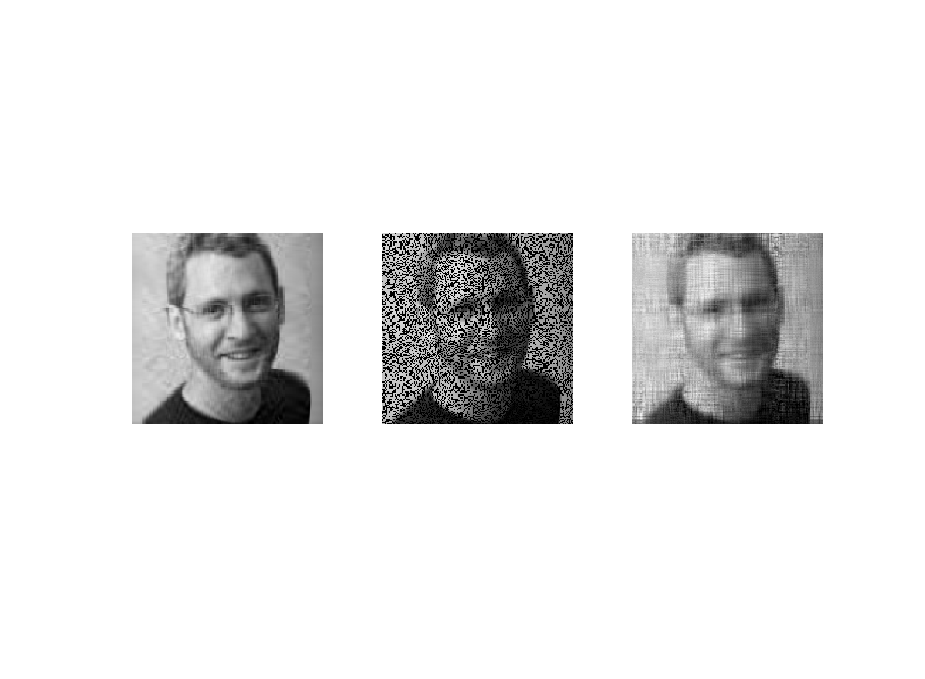
\includegraphics[trim = 55 100 40 100, clip, width=0.99\linewidth]{figs/MPF.eps}
	\caption{Low rank image reconstruction using the DualCG method. {\bf Left:} Original low rank ($= 20$) image. {\bf Middle:} Sparse Image with 40\% of entries missing. {\bf Right:} Reconstructed image with $\tau = 90$ and $\ell = 20$. }\label{fig:MPF}
\end{figure*}

We finally test the DualCG and sketchyCG algorithms on some real-world data.
\textcolor{red}{The dataset we use is the data called MovieLens 10K datasets obtained from \cite{10.1145/2827872} for ??? users rating ??? movie titles from 1 to 5.
	The sparsity of this data set is ???.}
Figure \ref{fig:Movielens10k} shows optimality gap convergence results applied to MovieLens 10K dataset, fixing the hyperparameters $\ell =1$ and $\tau = 20$. The results show that using DualCGM, the optimality gap converges in much fewer iterations in comparison to SketchyCG. Although the trend in SketchyCG seems to be much smoother. The $\rm NMAE$ for the DualCG and SketchyCG were $ 0.0512$ and $0.0534$ respectively.
\begin{figure*}[!htb]
	\centering
	\includegraphics[width=0.40\linewidth]{figs/SketchyCGM-10k.pdf}
	\includegraphics[width=0.40\linewidth]{figs/DualCGM-10k.pdf}
	\caption{Optimality gap of the SketchyCG and DualCG algorithms when applied to the matrix completion problem using the MovieLens 10K dataset.}
	\label{fig:Movielens10k}
\end{figure*}

We also applied the DualCG algorithm to the extension of MovieLens 10K dataset, called  MovieLens 100K dateset.
This dataset has
The only


\section{Conclusion} \label{ sec:conclusion }

In this work, we have provided a comprehensive review of the conditional gradient method, commonly referred to as the Frank-Wolfe algorithm, and its variants. These methods have been shown to be particularly robust in addressing a variety of optimization challenges. Specifically, we focused on two significant applications: the lasso problem, which is central to sparse regression in statistics, and the matrix completion problem, a key component in collaborative filtering and recommendation systems.

The conditional gradient method, with its inherent simplicity and efficiency, has proven to be highly effective for solving lasso problems, especially in high-dimensional settings where traditional methods struggle.

Similarly, in the realm of matrix completion, the conditional gradient method has demonstrated remarkable performance. The ability of the conditional gradient method to handle large-scale matrices efficiently makes it an attractive choice for such applications.

Furthermore, we explored storage-efficient variants of the conditional gradient method. Our comparative analysis revealed that these storage-efficient methods not only maintain the efficacy of the standard algorithm but also significantly reduce memory usage, making them ideal for large-scale problems.

Additionally, our study delved into the convergence properties of these methods. We demonstrated that the conditional gradient method offers guaranteed convergence rates, which is crucial for ensuring the reliability and predictability of the algorithm in practical applications.

In summary, the conditional gradient method and its variants stand out as powerful tools in optimization. Their ability to handle large-scale problems with efficiency and their robustness in various applications underscore their importance in both theoretical research and practical implementation. Future work may involve extending these methods and exploring their integration with other optimization techniques.


\bibliographystyle{plain}
\bibliography{bib.bib}

\end{document}
